\exo{Décrire chaque figure avec une phrase puis donner la notation mathématique.}

\begin{tabularx}{\linewidth}{|*{3}{>{\centering\arraybackslash}X|}}
	\hline
	Figure \no{1} & Figure \no{2} & Figure \no{3} \\
	\hline	
		\begin{tikzpicture}[scale=.5]
		\NoAutoSpacing
		\tkzDefPoints{0/0/M,4/2/N}
	    \tkzDrawSegment[|-|](M,N)
	    \tkzLabelPoints[above=.1](M,N)
	    \tkzDrawSegment[add=0 and .3](M,N)
		\end{tikzpicture}
	&
	    \begin{tikzpicture}[scale=.5]
	    \NoAutoSpacing
	    \tkzDefPoints{0/0/E,4/2/F}
	    \tkzDrawSegment[|-|](E,F)
	    \tkzLabelPoints[above=.1](E,F)
	    \tkzDrawSegment[add=.3 and .3](F,E)
		\end{tikzpicture}
	&
		\begin{tikzpicture}[scale=.5]
		\NoAutoSpacing
	    \tkzDefPoints{0/0/A,4/2/B}
	    \tkzDrawSegment[|-|](A,B)
	    	\tkzLabelPoints[above=.1](A,B)
		\end{tikzpicture}
 \\
	\hline
\end{tabularx}

\exo{Pour chacune des constructions, les points $A$, $B$ et $C$ étant déjà placés, écrire un texte pour décrire les $3$ \textit{traits} avec les notations mathématiques.}


\begin{center}
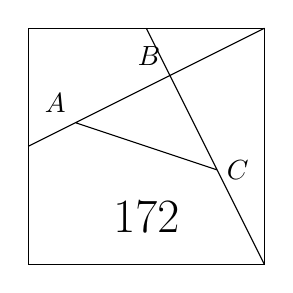
\begin{tikzpicture}[scale=.6] \NoAutoSpacing
		\draw (0,0) rectangle (5,5);	
		\draw (1,3) node [above left] {$A$};
		\draw (3,4) node [above left] {$B$};
		\draw (4,2) node [right] {$C$};
		\draw 	(0,2.5) -- (5,5) 
				(1,3) -- (4,2)
				(2.5,5) -- (5,0);
		\draw (2.5,1) node {\LARGE{\ding{172}}};
\end{tikzpicture}
	\hspace{3cm}
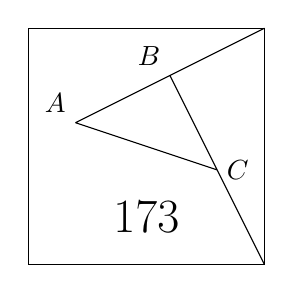
\begin{tikzpicture}[scale=.6] \NoAutoSpacing
		\draw (0,0) rectangle (5,5);	
		\draw (1,3) node [above left] {$A$};
		\draw (3,4) node [above left] {$B$};
		\draw (4,2) node [right] {$C$};
		\draw 	(1,3) -- (5,5) 
				(1,3) -- (4,2)
				(3,4) -- (5,0);
		\draw (2.5,1) node {\LARGE{\ding{173}}};
\end{tikzpicture} 	
\end{center}

\exo{}

\begin{itemize}
	\item Placer 4 points non alignés $A$, $B$, $C$, $D$.
	\item Tracer $[CA)$.
	\item Tracer $(AD)$.
	\item Tracer $[BD]$.
\end{itemize}